
\chapter{Theory of limits}
\label{ch:3}

%13
\section{Limit of a variable}
\label{sec:13}

If a variable $v$ takes on successively a series of values 
that approach nearer and nearer to a constant value $L$ 
in such a manner that $| v - L |$ becomes and remains 
less than any assigned arbitrarily small positive quantity, 
then $v$ is said to approach the limit $L$, or to converge 
to the limit $L$. Symbolically this is written

\[
\lim_{v = L},\ \ {\rm or},\ \ \lim_{v \rightarrow L}. 
\]

The following familiar examples illustrate what is meant:

\begin{enumerate}
\item
%(1) 
As the number of sides of a regular inscribed polygon is 
indefinitely increased, the limit of the area of the polygon 
is the area of the circle. In this case the variable is always 
less than its limit.

\item
%(2) 
Similarly, the limit of the area of the circumscribed polygon 
is also the area of the circle, but now the variable is 
always greater than its limit.

\item
%(3) 
Consider the series
\begin{equation}
%(A) 
1 - \frac{1}{2} + \frac{1}{4} - \frac{1}{8} + \cdots
\label{eqn:A}
\end{equation}
The sum of any even number $(2n)$ of the first terms of this series is

\begin{equation}
\begin{array}{ll}
 S_{2n}	&= 1 - \frac{1}{2} + \frac{1}{4} - \frac{1}{8} + \cdots 
+ \frac{1}{2^{2n - 2}} - \frac{1}{2^{2n - 1}}\\
&= \frac{\frac{1}{2^{2n}} - 1}{-\frac{1}{2} - 1} \\
&= \frac{2}{3} - \frac{1}{3 \cdot 2^{2n - 1}},
\end{array}
\label{eqn:B}
\end{equation}
by item 6, Ch. \ref{ch:1}, \S \ref{sec:1}.
Similarly, the sum of any odd number $(2n + 1)$ of the first terms of 
the series is

\begin{equation}
\begin{array}{ll}
S_{2n + 1} 	&
= 1 - \frac{1}{2} + \frac{1}{4} - \frac{1}{8} + 
\cdots - \frac{1}{2^{2n - 1}} + \frac{1}{2^{2n}}\\
&= \frac{-\frac{1}{2^{2n + 1}} - 1}{-\frac{1}{2} - 1} \\
&= \frac{2}{3} + \frac{1}{3 \cdot 2^{2n}},
\end{array}
\label{eqn:C}
\end{equation}
again by item 6, Ch. \ref{ch:1}, \S \ref{sec:1}.

Writing (\ref{eqn:B}) and (\ref{eqn:C}) in the forms

\[
 \frac{2}{3} - S_{2n} 
= \frac{1}{3 \cdot 2^{2n - 1}}, 
\ \ \ \ \ S_{2n + 1} - \frac{2}{3} 
= \frac{1}{3 \cdot 2^{2n}}
\]
we have 
\[
\lim_{n \to \infty} \left ( \frac{2}{3} - S_{2n} \right ) 	
= \lim_{n \to \infty} \frac{1}{3 \cdot 2^{2n - 1}} = 0,
\]
and 

\[
\lim_{n \to \infty} \left ( S_{2n + 1} - \frac{2}{3} \right ) 	
= \lim_{n \to \infty} \frac{1}{3 \cdot 2^{2n}} = 0.
\]
Hence, by definition of the limit of a variable, it is seen 
that both $S_{2n}$ and $S_{2n + 1}$ are variables approaching 
$\frac{2}{3}$ as a limit as the number of terms increases without limit.

Summing up the first two, three, four, etc., terms of (\ref{eqn:A}), 
the sums are found by ((\ref{eqn:B}) and ((\ref{eqn:C}) to 
be alternately less and greater than $\frac{2}{3}$, illustrating 
the case when the variable, in this case the sum of the terms 
of ((\ref{eqn:A}), is alternately less and greater than its limit.
\end{enumerate}

In the examples shown the variable never reaches its limit. 
This is not by any means always the case, for from the definition 
of the limit of a variable it is clear that the essence of the 
definition is simply that the numerical value of the difference 
between the variable and its limit shall ultimately become and 
remain less than any positive number we may choose, however small.

\begin{example}
%(4) 
As an example illustrating the fact that the variable may 
reach its limit, consider the following. Let a series of regular 
polygons be inscribed in a circle, the number of sides increasing 
indefinitely. Choosing anyone of these, construct. the circumscribed 
polygon whose sides touch the circle at the vertices of the inscribed
polygon. Let $p_n$ and $P_n$ be the perimeters of the inscribed and 
circumscribed polygons of $n$ sides, and $C$ the circumference 
of the circle, and suppose the values of a variable $x$ to be as follows:

\[
 P_n,\ \  p_{n + 1},\ \  C,\ \  P_{n + 1},\ \  p_{n + 2},\ \  C,\ \  P_{n + 2},
\ \ \ \ {\rm etc.}
\]
Then, evidently,

\[
    \lim_{x \to \infty} x = C
\]
and the limit is reached by the variable, every third value of the 
variable being $C$.
\end{example}

%14
\section{Division by zero excluded}
\label{sec:14}

$\frac{0}{0}$ is indeterminate. For the quotient of two numbers 
is that number which multiplied by the divisor will give 
the dividend. But any number whatever multiplied by zero 
gives zero, and the quotient is indeterminate; that is, 
any number whatever may be considered as the quotient, a 
result which is of no value.

$\frac{a}{0}$ has no meaning, $a$ being different from zero, 
for there exists no number such that if it be multiplied by zero, 
the product will equal $a$.

Therefore division by zero is not an admissible operation.

Care should be taken not to divide by zero inadvertently. The following 
fallacy is an illustration.
Assume that 
\[
	a 	= b.
\]
Then evidently 	
\[
ab = a^2.
\]
Subtracting $b^2$,
\[
 ab-b^2 	= a^2-b^2.
\]
Factoring, 	
\[
b(a-b) 	= (a + b)(a-b).
\]
Dividing by %a - b%, 	
\[
b = a + b.
\]
But 	$a 	= b$,
therefore $b 	= 2b$,
or, 	$1 	= 2$.
The result is absurd, and is caused by the fact that we divided by 
$a-b = 0$.

%15
\section{Infinitesimals}
\label{sec:15}

A variable $v$ whose limit is zero is called an {\it 
infinitesimal}\footnote{Hence a constant, no matter how small 
it may be, is not an infinitesimal.}.
This is written
\[
    \lim_{v = 0}, \ {\rm or},\ \lim_{v\rightarrow 0},
\]
and means that the successive numerical values of $v$ ultimately 
become and remain less than any positive number however small. 
Such a variable is said to become indefinitely small or to ultimately vanish.

If   $\lim v = l$, then $\lim (v-l) = 0$;
that is, the difference between a variable and its limit is an infinitesimal.

Conversely, if the difference between a variable and a 
constant is an infinitesimal, then the variable approaches the 
constant as a limit.

%16
\section{The concept of infinity ($\infty$)}

If a variable $v$ ultimately becomes and remains greater than 
any assigned positive number, however large, we say $v$ 
``increases without limit'', and write

\[
\lim_{v = +\infty},\ {\rm or},\ \lim_{v\rightarrow +\infty},  \ {\rm or},
\ v\rightarrow +\infty.
\]
If a variable $v$ ultimately becomes and remains algebraically 
less than any assigned negative number, we say 
``$v$ decreases without limit'', and write

\[
\lim_{v = -\infty},\ {\rm or},\ \lim_{v\rightarrow -\infty},  \ {\rm or},
\ v\rightarrow -\infty.
\]
If a variable $v$ ultimately becomes and remains in numerical value 
greater than any assigned positive number, however large, 
we say $v$, in numerical value, ``increases without limit'', or 
$v$ becomes infinitely great\footnote{On account of the notation 
used and for the sake of uniformity, the expression 
$ v\rightarrow +\infty$ is sometimes read ``$v$ approaches the limit 
plus infinity''. Similarly, $ v\rightarrow -\infty$ is read ``$v$ 
approaches the limit minus infinity'', and $ v\rightarrow \infty$
is read ``$v$, in numerical value, approaches the limit infinity''.
While the above notation is convenient to use in this connection, 
the student must not forget that infinity is not a limit in the sense 
in which we defined it in \S \ref{sec:14}, for infinity is 
not a number at all.}, and write

\[
\lim_{v = \infty},\ {\rm or},\ \lim_{v\rightarrow \infty},  \ {\rm or},
\ v\rightarrow \infty.
\]
Infinity ($\infty$) is not a number; it simply serves to characterize 
a particular mode of variation of a variable by virtue of which 
it increases or decreases without limit.

%17
\section{Limiting value of a function}

Given a function $f(x)$. If the independent variable $x$ takes on 
any series of values such that

\[
\lim x = a,
\]
and at the same time the dependent variable $f(x)$ takes on a 
series of corresponding values such that

\[
\lim f(x) = A,
\]
then as a single statement this is written

\[
  \lim_{x \to a} f(x) = A. 
\]

Here is an example of a limit using \sage:

\vskip .2in

\begin{Verbatim}[fontsize=\scriptsize,fontfamily=courier,fontshape=tt,frame=single,label=\sage]

sage: limit((x^2+1)/(2+x+3*x^2),x=infinity)
1/3

\end{Verbatim}

\vskip .1in
\noindent
This tells us that 
$\lim_{x \to \infty} \frac{x^2+1}{2+x+3*x^2}=\frac{1}{3}$.

%18
\section{Continuous and discontinuous functions}
\label{sec:18}

A function $f(x)$ is said to be {\it continuous} for $x = a$ if 
the limiting value of the function when $x$ approaches the limit $a$ 
in any manner is the value assigned to the function for $x = a$. 
\index{continuous}
In symbols, if
\[
    \lim_{x \to a} f(x) = f(a),
\]
then $f(x)$ is continuous for $x = a$.

The function is said to be {\it discontinuous} for $x = a$ 
if this condition is not satisfied. For example, if
\index{discontinuous}

\[
    \lim_{x \to a} f(x) = \infty,
\]
the function is discontinuous for $x = a$.

The attention of the student is now called to the following cases 
which occur frequently.

\noindent
{\bf CASE I}. 
As an example illustrating a simple case of a function continuous 
for a particular value of the variable, consider the function

\[
    f(x) = \frac{x^2 - 4}{x - 2}.
\]
For $x = 1$, $f(x) = f(l) = 3$. Moreover, if $x$ approaches the limit 
$1$ in any manner, the function $f(x)$ approaches $3$ as a limit. 
Hence the function is continuous for $x = 1$.

\noindent
{\bf CASE II}. 
The definition of a continuous function assumes that the function 
is already defined for $x = a$. If this is not the case, however, 
it is sometimes possible to assign such a value to the function 
for $x = a$ that the condition of continuity shall be satisfied. 
The following theorem covers these cases.

\begin{theorem}
If $f(x)$ is not defined for $x = a$, and if

\[
    \lim_{x \to a} f(x) = B,
\]
then $f(x)$ will be continuous for $x = a$, if $B$ 
is assumed as the value of $f(x)$ for $x = a$. 
\end{theorem}

Thus the function

\[
    \frac{x^2 - 4}{x - 2}
\]
is not defined for $x = 2$ (since then there would be division by 
zero). But for every other value of $x$,

\[
    \frac{x^2 - 4}{x + 2} = x + 2;
\]
and 
\[
\lim_{x \to 2} (x + 2) 	= 4
\]
therefore $\lim_{x \to 2} \frac{x^2 - 4}{x - 2} 	= 4$.
Although the function is not defined for $x = 2$, if we % arbitrarily
assign it the value $4$ for $x = 2$, it then becomes continuous for this value.

A function $f(x)$ is said to be {\it continuous in an interval} when 
it is continuous for all values of $x$ in this interval\footnote{In 
this book we shall deal only with functions which are in general 
continuous, that is, continuous for all values of $x$, with the 
possible exception of certain isolated values, our results in 
general being understood as valid only for such values of $x$ 
for which the function in question is actually continuous. 
Unless special attention is called thereto, we shall as a rule 
pay no attention to the possibilities of such exceptional values 
of $x$ for which the function is discontinuous. The definition 
of a continuous function f(x) is sometimes roughly (but imperfectly) 
summed up in the statement that a small change in $x$ shall produce 
a small change in $f(x)$. We shall not consider functions having 
an infinite number of oscillations in a limited region.}.

%19
\section{Continuity and discontinuity of functions illustrated by their graphs}
\label{sec:19}


\begin{enumerate}
\item
%(1) 
Consider the function $x^2$, and let

\begin{equation}
 y = x^2
\label{eqn:III-A}
\end{equation}
If we assume values for x and calculate the corresponding values of y, 
we can plot a series of points. Drawing a smooth line free-hand through 
these points: a good representation of the general behavior of the 
function may be obtained. This picture or image of the function is 
called its {\it graph}. It is evidently the locus of all points satisfying 
equation (\ref{eqn:III-A}).
\index{graph}

\begin{figure}[h!]
\begin{minipage}{\textwidth}
\begin{center}
%\vspace{1.0 cm}
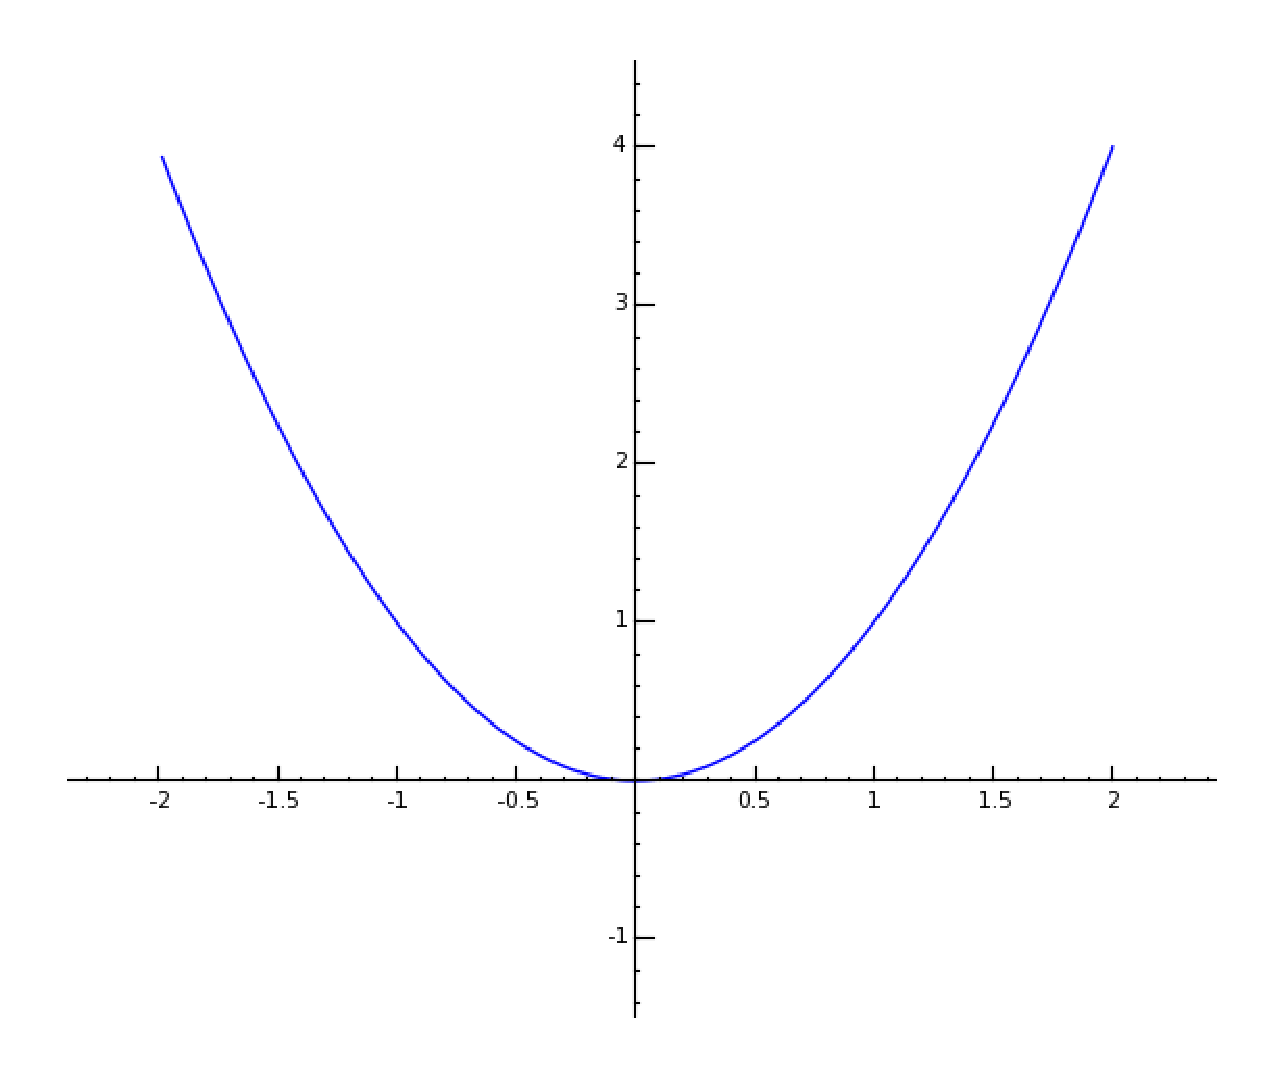
\includegraphics[height=5cm,width=3cm]{parabola.eps}
\end{center}
\end{minipage}
\caption{The parabola $y=x^2$.}
\label{fig:$x^2$}
\end{figure}
%sage: P = plot(x^2,-2,2)
%sage: show(P)

\noindent
It is very easy to create the above plot in \sage, as the example below 
shows:

\vskip .2in

\begin{Verbatim}[fontsize=\scriptsize,fontfamily=courier,fontshape=tt,frame=single,label=\sage]

sage: P = plot(x^2,-2,2)
sage: show(P)

\end{Verbatim}

\vskip .1in
\noindent
Such a series or assemblage of points is also called a {\it curve}. 
Evidently we may assume values of $x$ so near together as to bring 
the values of $y$ (and therefore the points of the curve) as near 
together as we please. In other words, there are no breaks in the 
curve, and the function $x^2$ is continuous for all values of $x$.

\item
%(2) 
\index{sin}
The graph of the continuous function $\sin x$, plotted by drawing the 
locus of $y = \sin\, x$,

\begin{figure}[h!]
\begin{minipage}{\textwidth}
\begin{center}
%\vspace{1.0 cm}
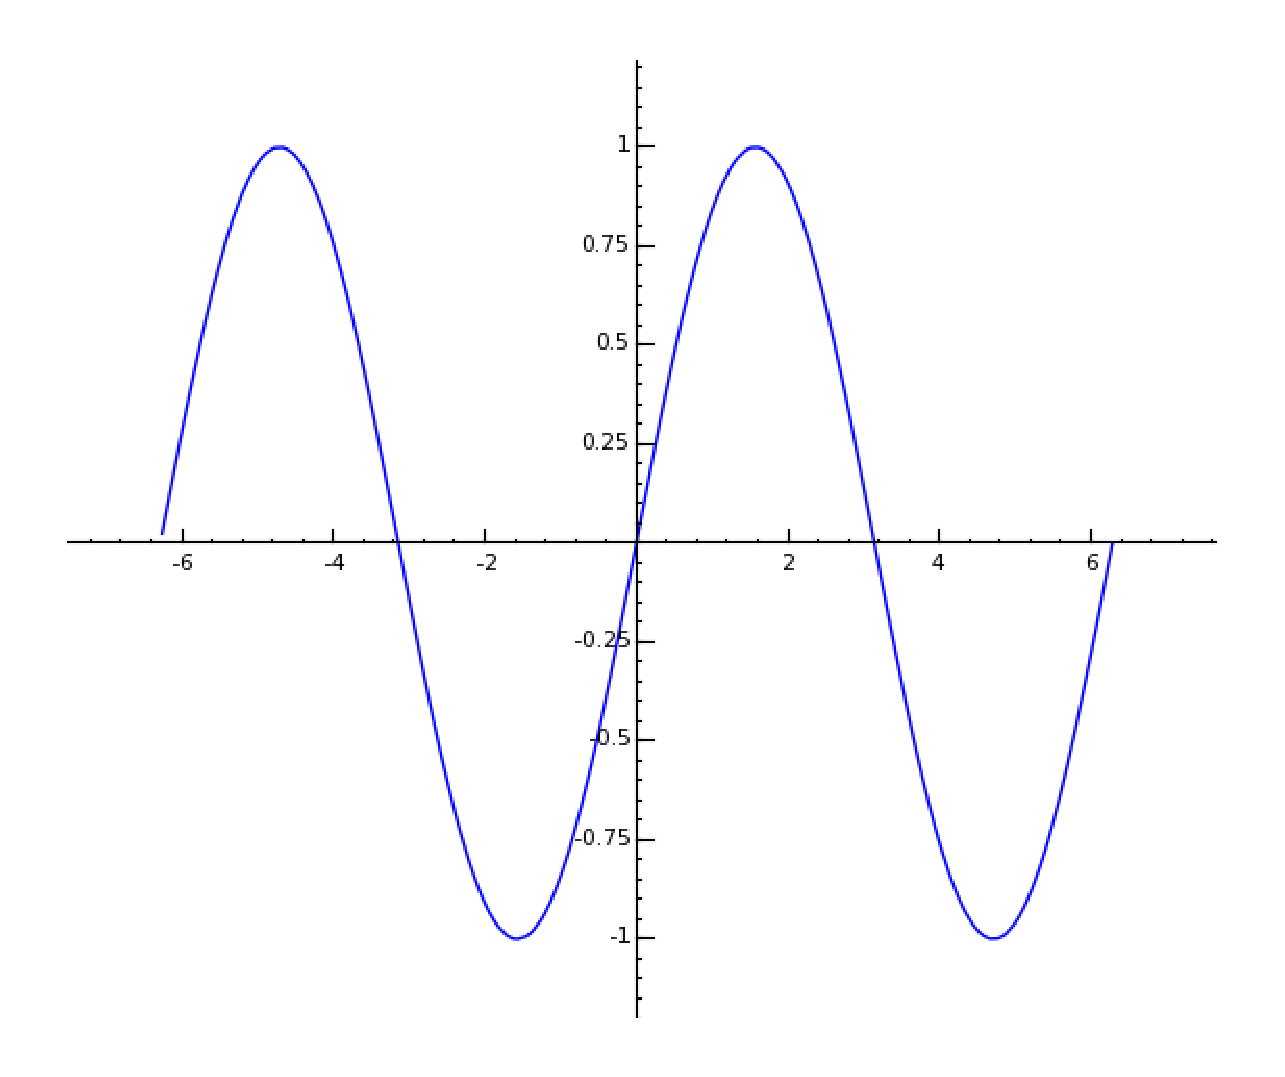
\includegraphics[height=3cm,width=9cm]{sine.eps}
\end{center}
\end{minipage}
\caption{The sine function.}
\label{fig:sin(x)}
\end{figure}
%sage: P = plot(sin(x),-2*pi,2*pi)
%sage: show(P)

It is seen that no break in the curve occurs anywhere.

\item
%(3) 
\index{exp}
The continuous function $exp(x) = e^x$ is of very frequent occurrence in 
the Calculus. If we plot its graph from

\[
    y= e^x, \qquad (e = 2.718\cdots),
\]
we get a smooth curve as shown. 

\begin{figure}[h!]
\begin{minipage}{\textwidth}
\begin{center}
%\vspace{1.0 cm}
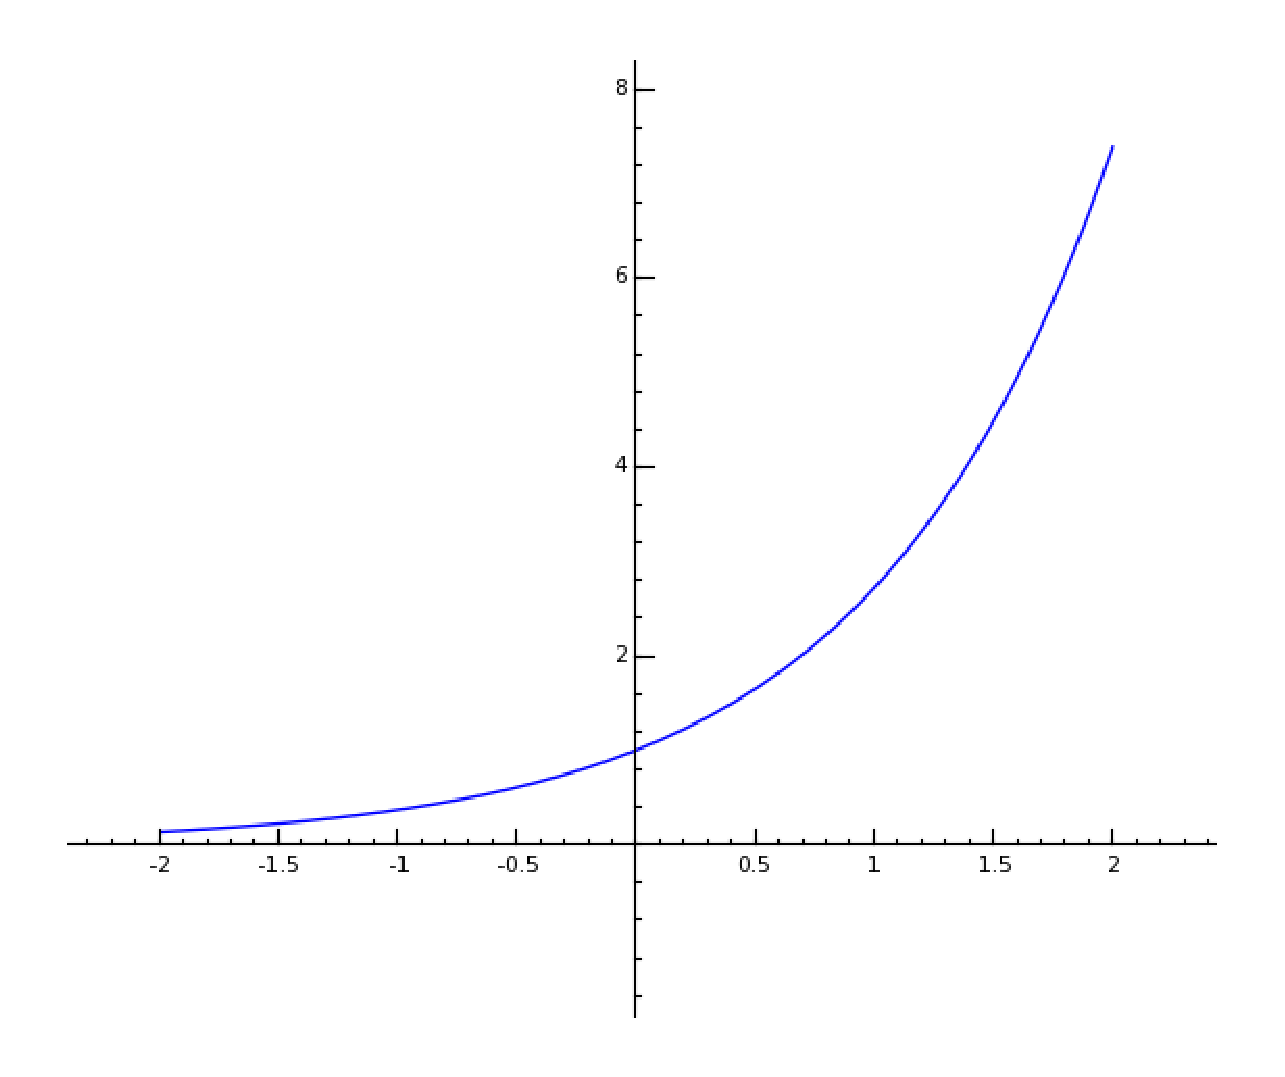
\includegraphics[height=5cm,width=5cm]{exp.eps}
\end{center}
\end{minipage}
\caption{The exponential function.}
\label{fig:exp(x)}
\end{figure}
%sage: P = plot(exp(x),-2,2)
%sage: show(P)

From this it is clearly seen that,

\begin{itemize}
\item[(a)] 
when $x = 0$,\ $\lim_{x \to 0} y (= \lim_{x \to 0} e^x) = 1$;

\item[(b)] 
when $x > 0$,\ $y (= e^x)$ is positive and increases as we pass 
towards the right from the origin;

\item[(c)] 
when $x < 0$,\ $y (= e^x)$ is still positive and decreases as 
we pass towards the left from the origin.

\end{itemize}

\item
%(4) 
\index{ln}
The function $\ln \, x = \log_e\ x$ is closely related to the last one 
discussed. In fact, if we plot its graph from

\[
    y = \log_e\ x,
\]
it will be seen that its graph has the same relation to 
$OX$ and $OY$ as the graph of $e^x$ has to $OY$ and $OX$.

\begin{figure}[h!]
\begin{minipage}{\textwidth}
\begin{center}
%\vspace{1.0 cm}
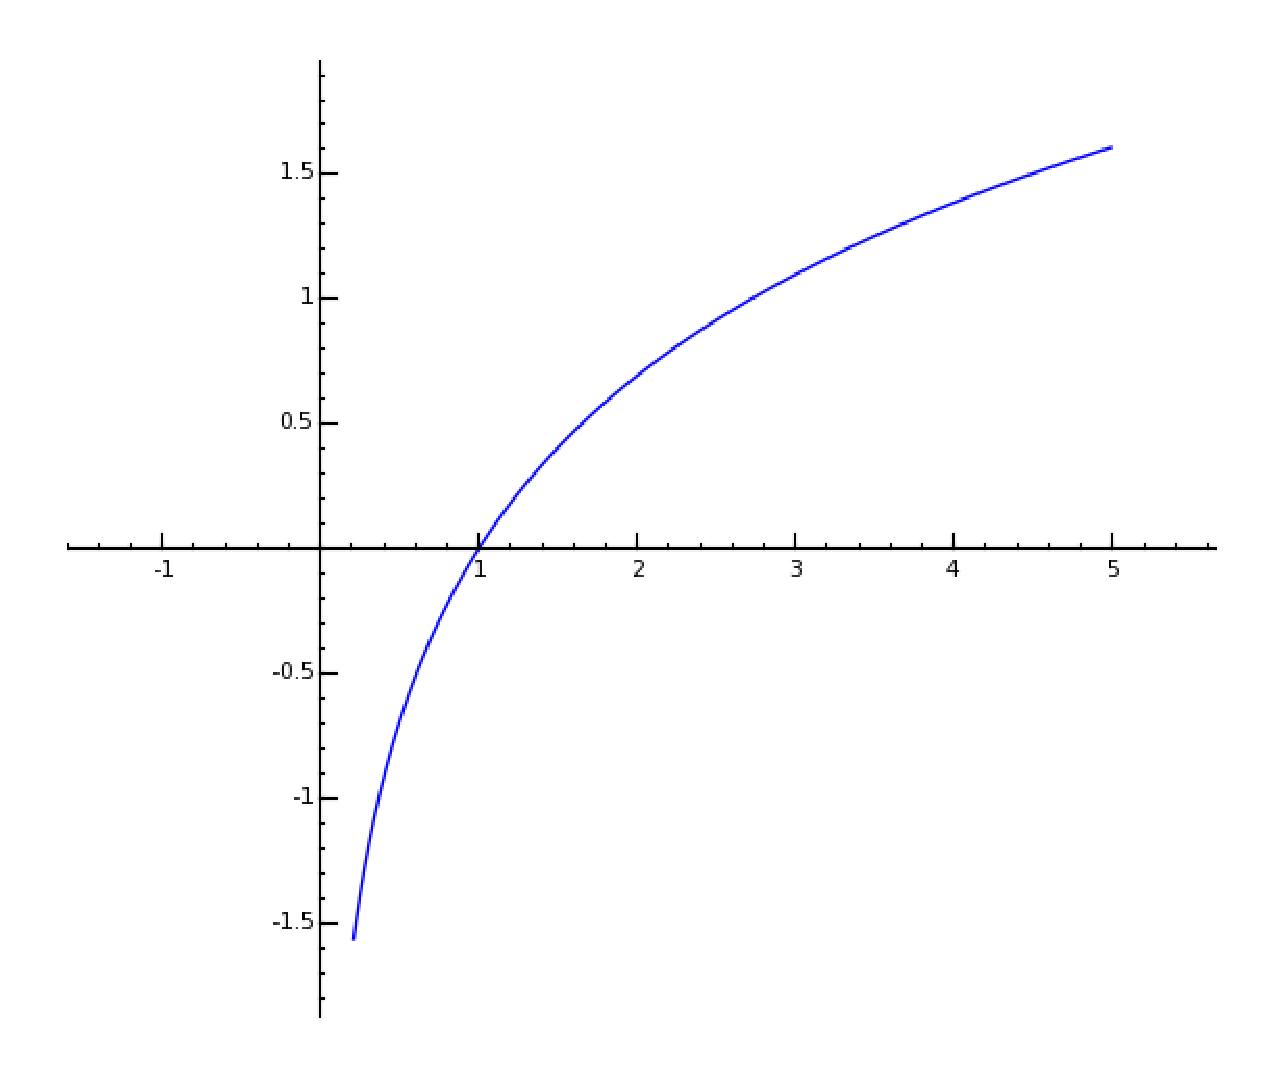
\includegraphics[height=4cm,width=7cm]{ln.eps}
\end{center}
\end{minipage}
\caption{The natural logarithm.}
\label{fig:ln(x)}
\end{figure}
%sage: P = plot(ln(x),1/5,5)
%sage: show(P)


Here we see the following facts pictured:

\begin{itemize}
\item[(a)] 
For $x = 1$,\ $\log_e\ x = \log_e\ 1 = 0$.

\item[(b)] 
For $x > 1$,\ $\log_e\ x$ is positive and increases as $x$ increases.

\item[(c)] 
For $1 > x > 0$,\ $\log_e\ x$ is negative and increases 
in numerical value as $x$, that is, $\lim_{x \to 0} \log\ x = -\infty$.

\item[(d)] 
For $x \le 0$,\ $\log_e\ x$ is not defined; hence the 
entire graph lies to the right of $OY$.

\end{itemize}


\item
%(5) 
Consider the function $\frac{1}{x}$, and set

\[
    y = \frac{1}{x}
\]
If the graph of this function be plotted, 
it will be seen 
that as $x$ approaches the value zero from the left 
(negatively), the points of the curve ultimately drop 
down an infinitely great distance, and as $x$ approaches the 
value zero from the right, the curve extends upward infinitely far.

%\newpage

\begin{figure}[h!]
\begin{center}
%\vspace{1.0 cm}
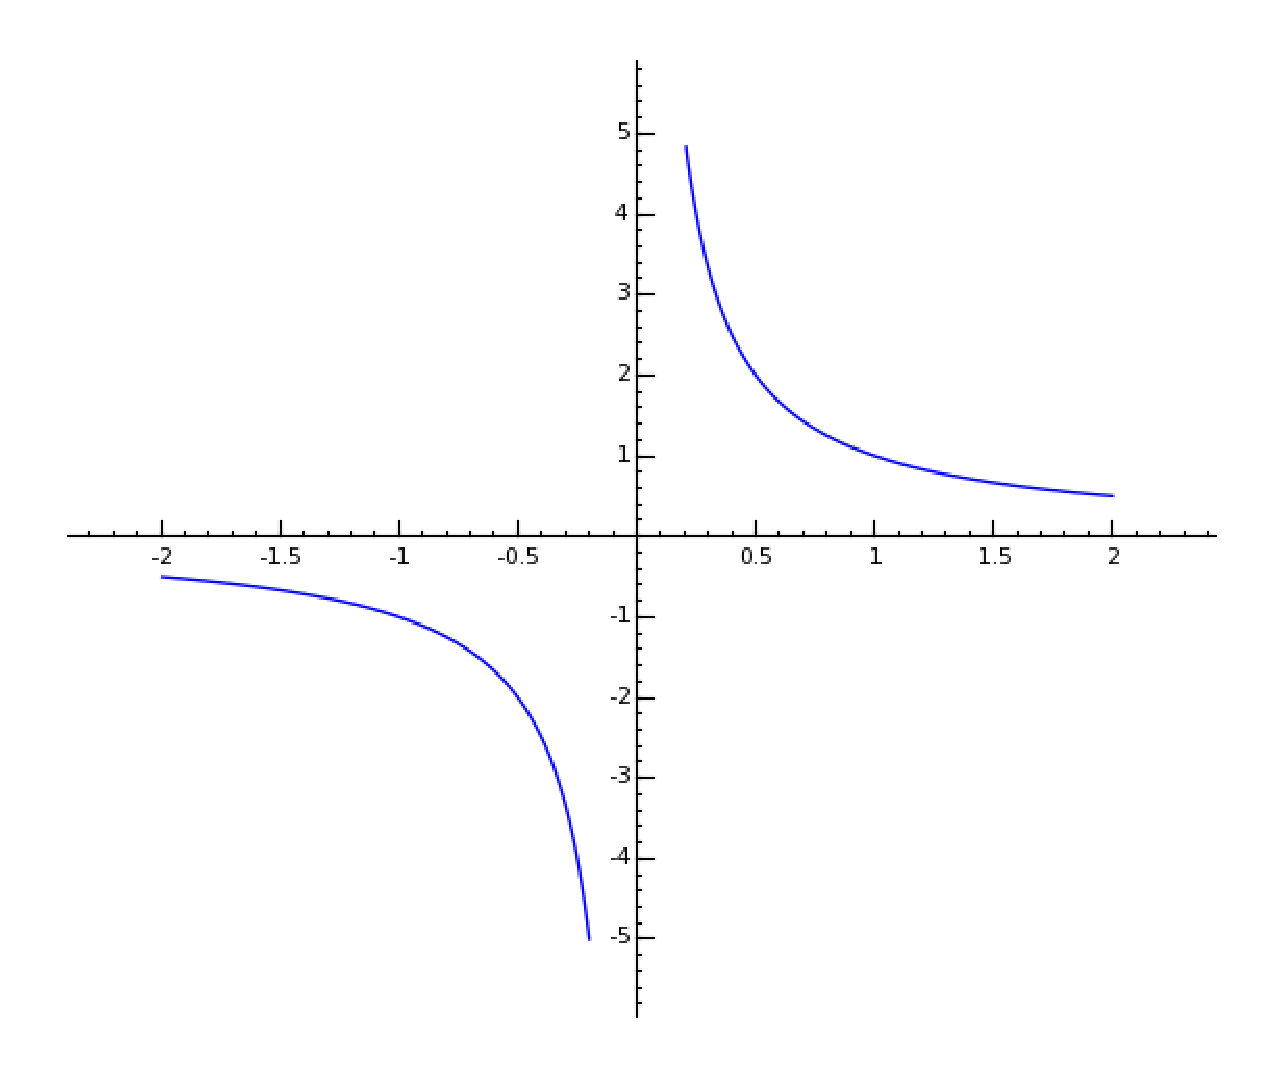
\includegraphics[height=5cm,width=7cm]{recip.eps}
\end{center}
\caption{The function $y=1/x$.}
\label{fig:1/x}
\end{figure}
%sage: P1 = plot(1/x,-2,-1/5)
%sage: P2 = plot(1/x,1/5,2)
%sage: show(P1+P2)

The curve then does not form a continuous branch from one side 
to the other of the axis of $y$, showing graphically that 
the function is discontinuous for $x = 0$, but continuous for all 
other values of $x$.


\item
%(6) 
From the graph (see Figure \ref{fig:2x/(1-x^2)}) of
\[
    y = \frac{2x}{1 - x^2}
\]
it is seen that the function $  \frac{2x}{1 - x^2}$
is discontinuous for the two values $x = \pm 1$, but 
continuous for all other values of $x$.


\begin{figure}[h!]
\begin{center}
%\vspace{1.0 cm}
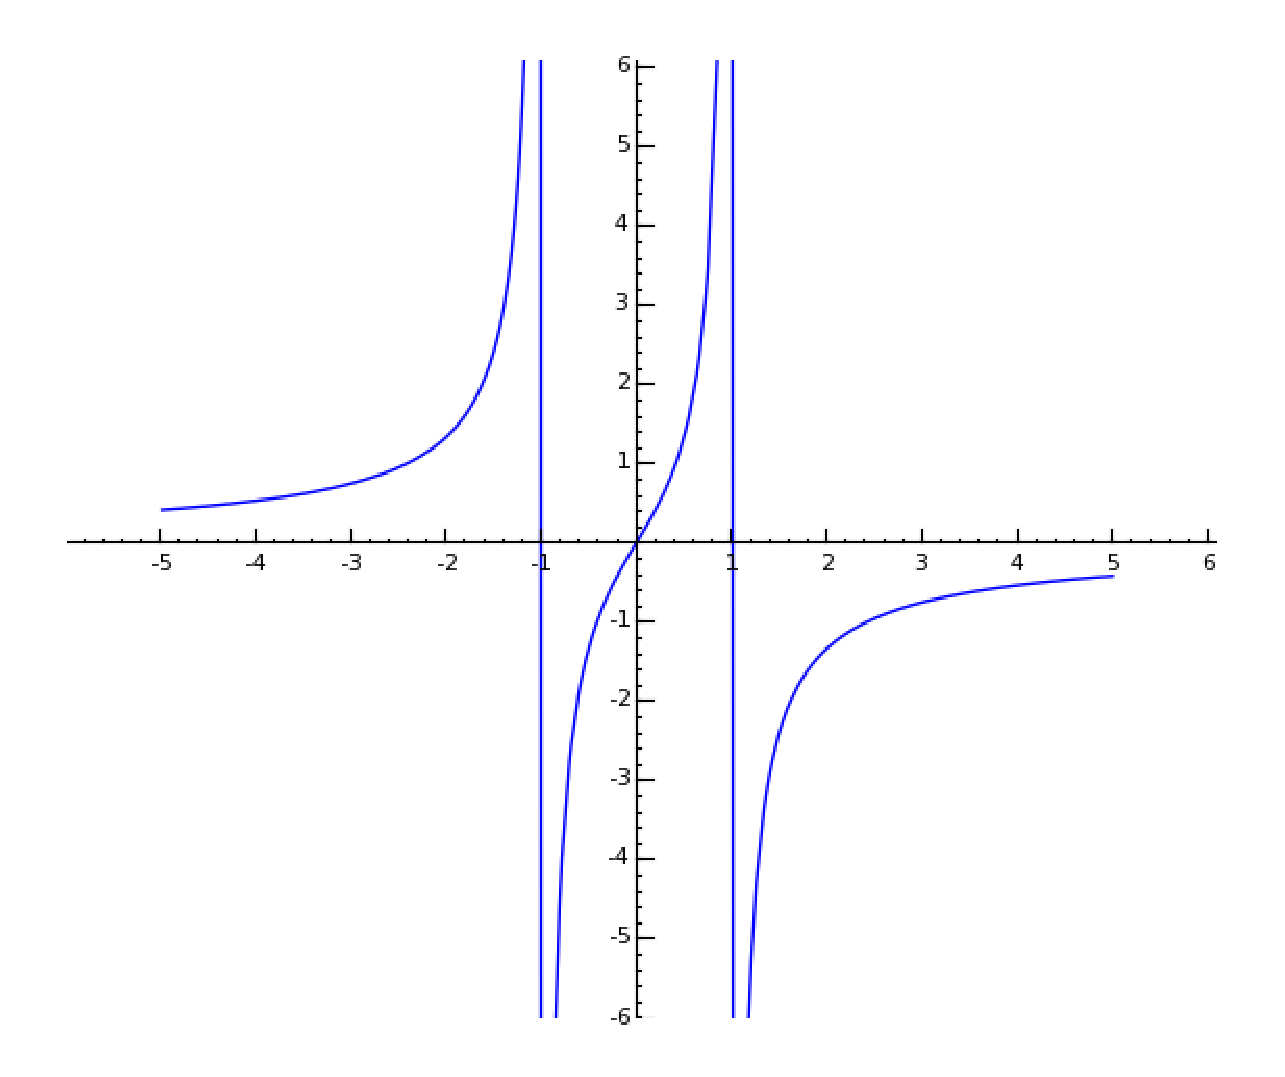
\includegraphics[height=7cm,width=7cm]{fcn6-III.eps}
\end{center}
\caption{The function $y=2x/(1-x^2)$.}
\label{fig:2x/(1-x^2)}
\end{figure}
%sage: P = plot(2*x/(1-x^2),-5,5)
%sage: show(P,ymin=-5,ymax=5)

\newpage

\item
%(7) 
\index{tan}
The graph of
\[
    y = \tan\ x
\]
shows that the function $\tan x$ is discontinuous for infinitely 
many values of the independent variable $x$, namely, 
$x = \frac{n\pi}{2}$, where $n$ denotes any odd positive or negative integer.

\begin{figure}[h!]
\begin{center}
%\vspace{1.0 cm}
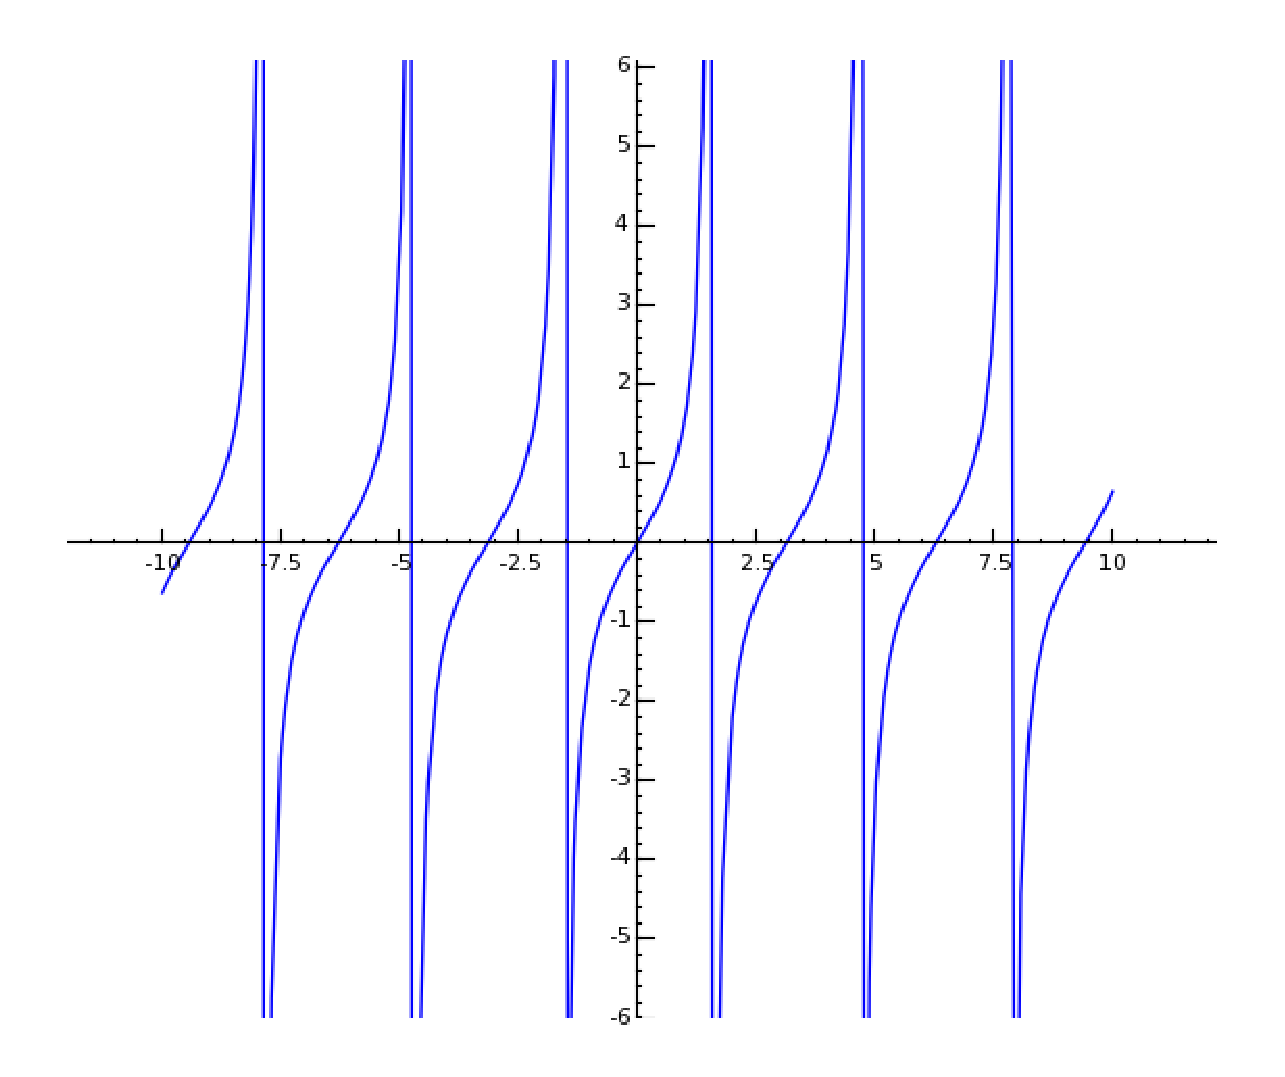
\includegraphics[height=5cm,width=8cm]{tan.eps}
\end{center}
\caption{The tangent function.}
\label{fig:tan(x)}
\end{figure}
%sage: P = plot(tan(x),-10,10)
%sage: show(P,ymin=-5,ymax=5)


\item
%(8) 
\index{arctan}
The function $\arctan\ x$
has infinitely many values for a given value of $x$, the graph of equation
\[
    y = \arctan\ x 
\]
consisting of infinitely many branches.

\begin{figure}[h!]
\begin{center}
%\vspace{1.0 cm}
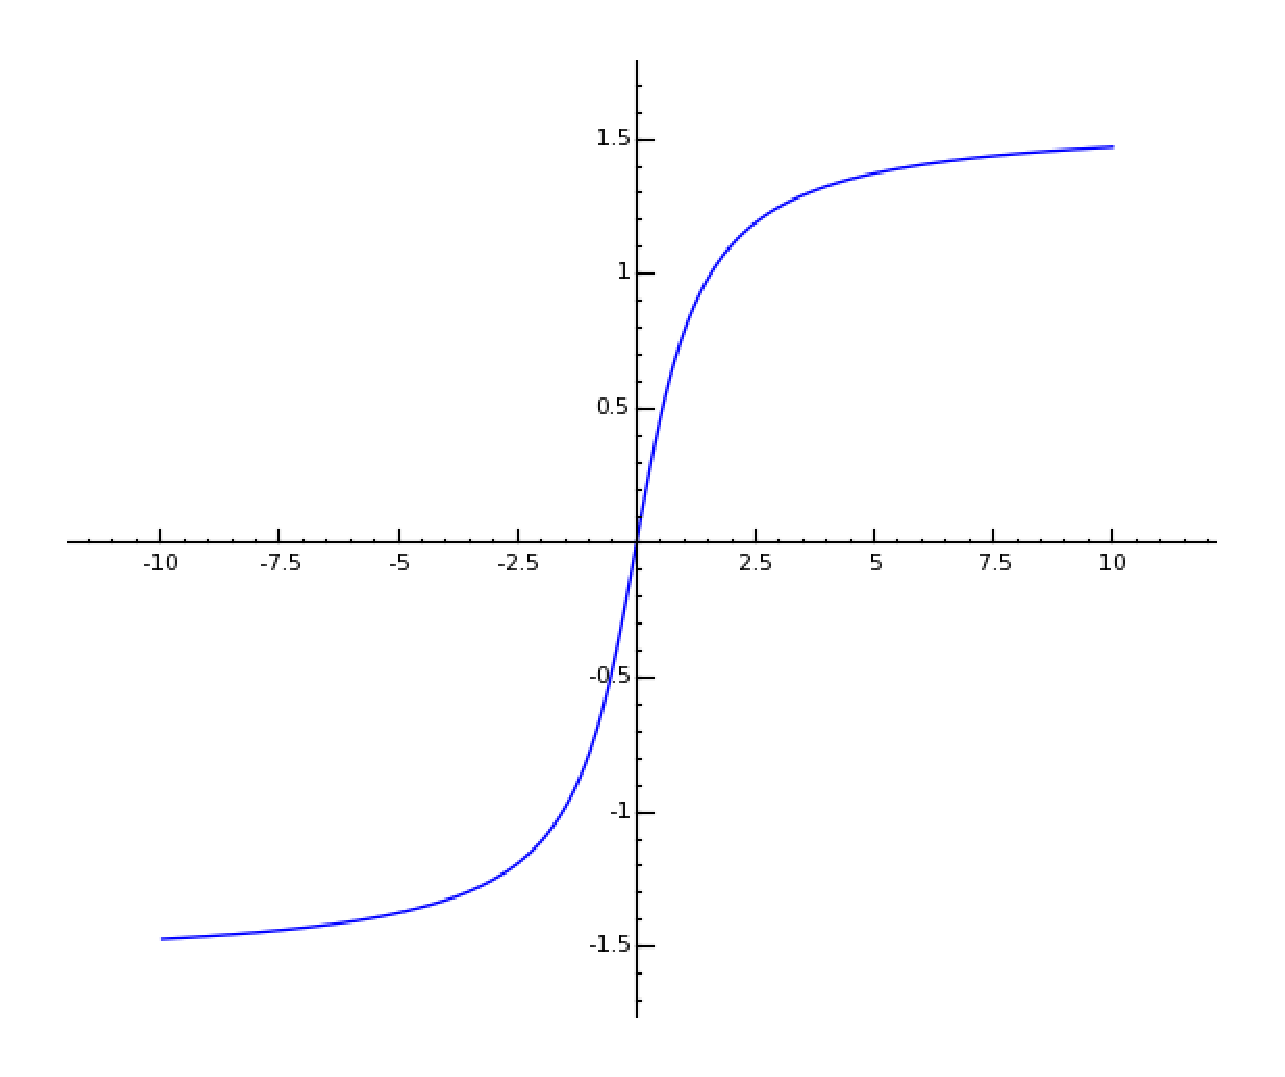
\includegraphics[height=4cm,width=8cm]{arctan.eps}
\end{center}
\caption{The arctangent (or inverse tangent) function.}
\label{fig:arctan(x)}
\end{figure}
%sage: P = plot(atan(x),-10,10)
%sage: show(P)

If, however, we confine ourselves to any single branch, the 
function is continuous. For instance, if we say that $y$ shall 
be the arc of smallest numerical value whose tangent is $x$, 
that is, $y$ shall take on only values between $-\frac{\pi}{2}$ 
and $\frac{\pi}{2}$, then we are limited to the branch passing 
through the origin, and the condition for continuity is satisfied.

\item
%(9) 
Similarly, $\arctan \frac{1}{x}$, is found to be a many-valued 
function. Confining ourselves to one branch of the graph of

\[
    y = \arctan\ \frac{1}{x}, 
\]
we see that as $x$ approaches zero from the left, 
$y$ approaches the limit $-\frac{\pi}{2}$, and as 
$x$ approaches zero from the right, $y$ approaches the limit 
$+\frac{\pi}{2}$. Hence the function is discontinuous when 
$x = 0$. Its value for $x = 0$ can be assigned at pleasure.

\begin{figure}[h!]
\begin{center}
%\vspace{1.0 cm}
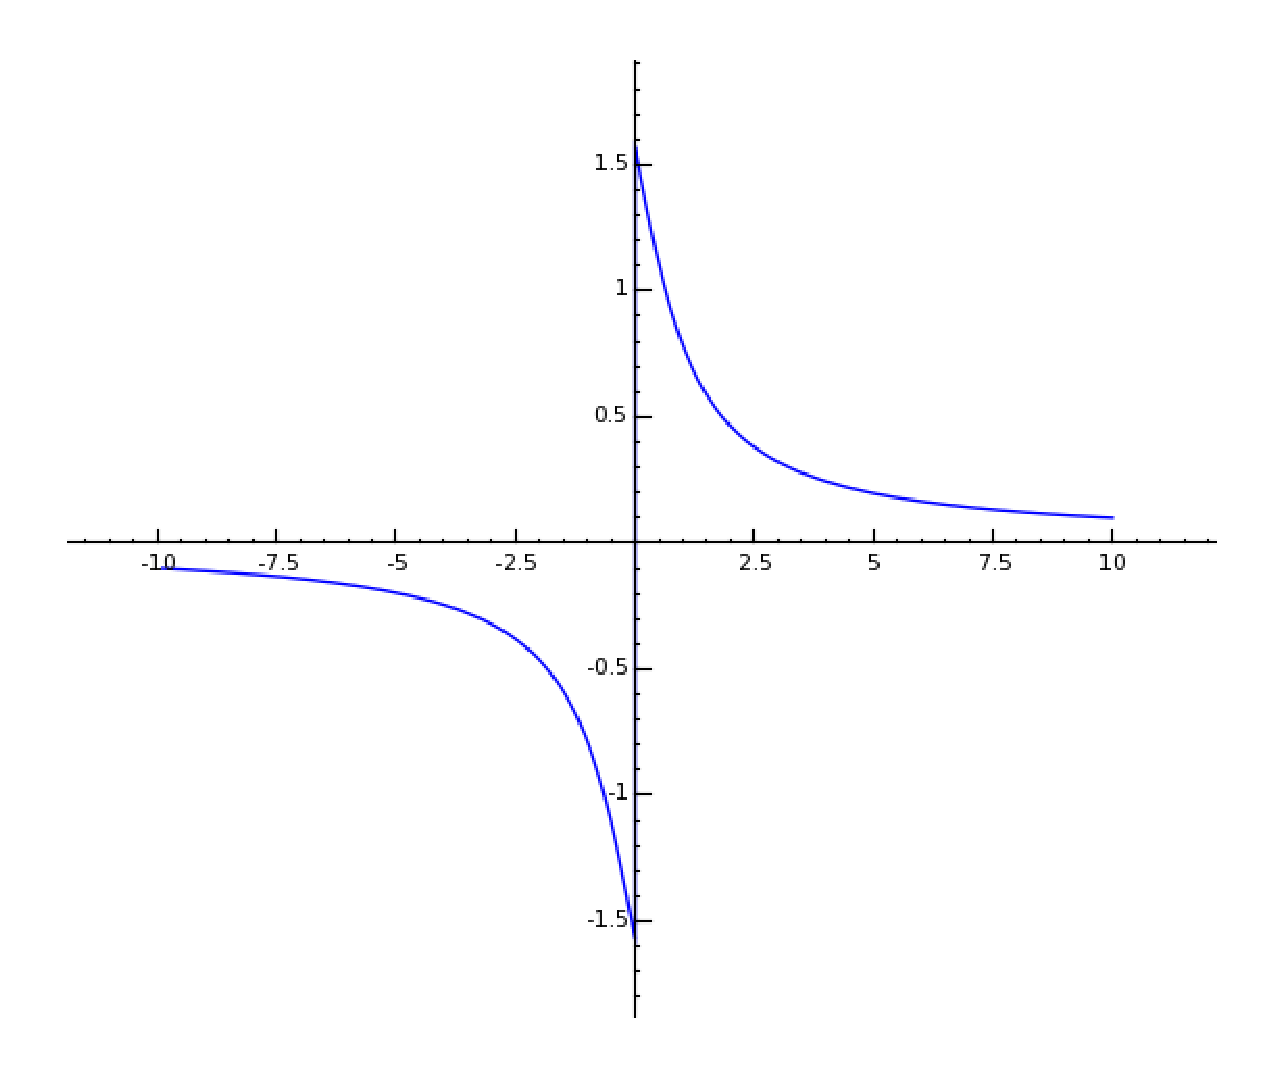
\includegraphics[height=4cm,width=8cm]{arctan1ox.eps}
\end{center}
\caption{The function $y=\arctan(1/x)$.}
\label{fig:arctan(1/x)}
\end{figure}
%sage: P = plot(atan(1/x),-10,10)
%sage: show(P)

\item
%% new
A {\it piecewise defined function}
\index{function! piecewise defined}
is one which is defined by different rules on 
different non-overlapping invervals. For example,

\[
f(x) = 
\left\{
\begin{array}{ll}
-1, & x<-\pi/2,\\
\sin(x), &\pi/2\leq x\leq \pi/2,\\
1, &\pi/2<x.
\end{array}
\right.
\]
is a continuous piecewise defined function.

\begin{figure}[h!]
\begin{center}
%\vspace{1.0 cm}
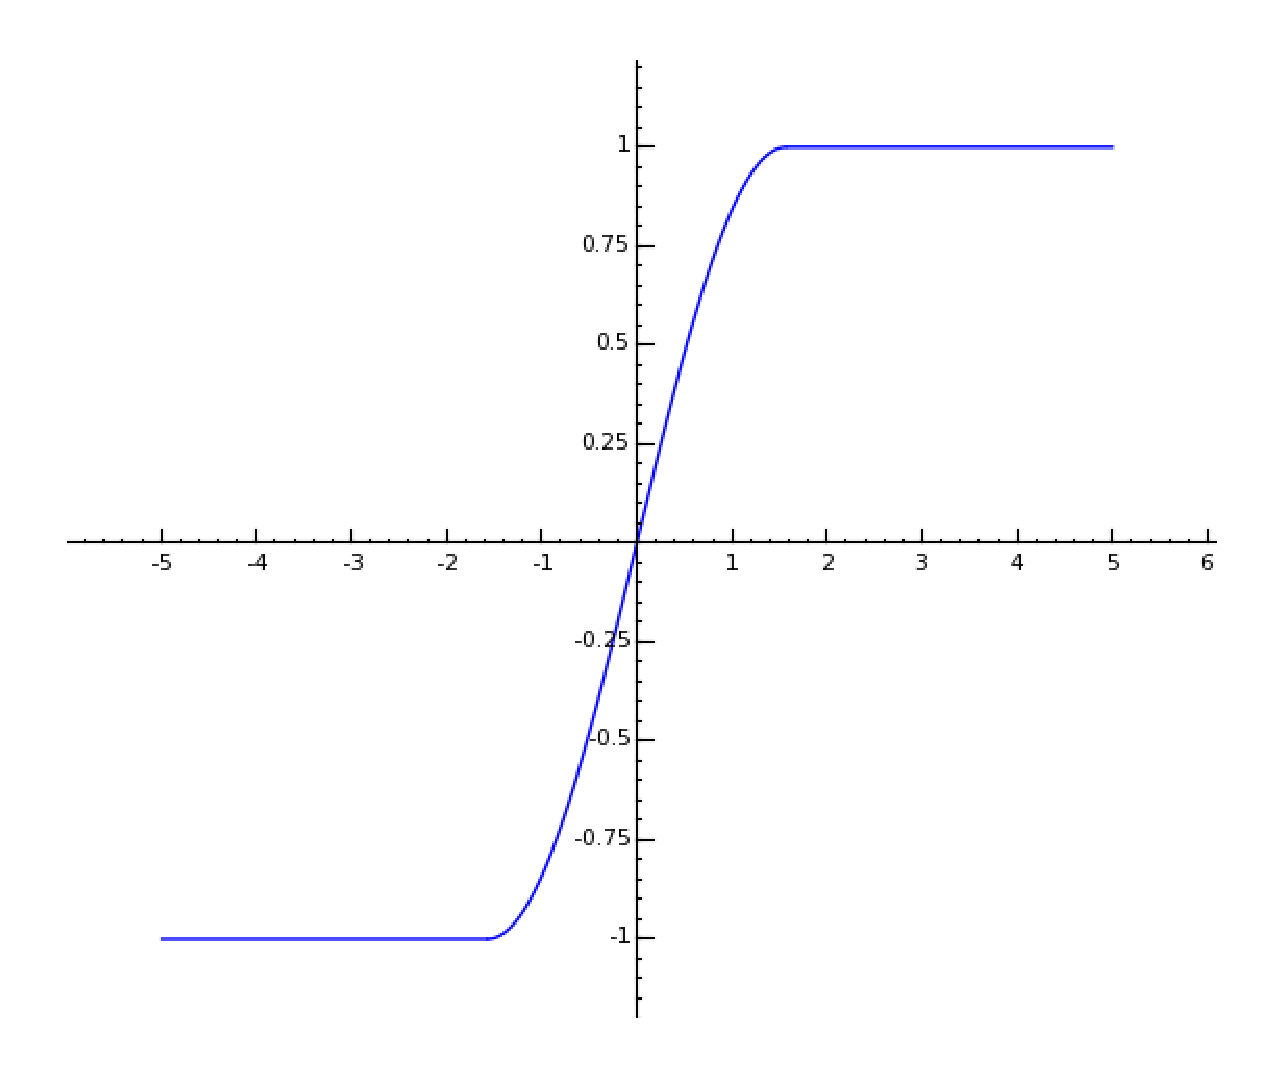
\includegraphics[height=4cm,width=8cm]{piecewise.eps}
\end{center}
\caption{A piecewise defined function.}
\label{fig:piecewise}
\end{figure}
%sage: f1 = lambda x: -1
%sage: f2 = lambda x: sin(x)
%sage: f3 = lambda x: 1
%sage: f = piecewise([[(-5,-pi/2),f1],[(-pi/2,pi/2),f2],[(pi/2,5),f3]])
%sage: P = f.plot()
%sage: show(P)

For example,

\[
f(x) = 
\left\{
\begin{array}{ll}
-1, & x<-2,\\
3, &-2\leq x\leq 3,\\
2, &3<x.
\end{array}
\right.
\]
is a discontinuous piecewise defined function, with 
jump discontinuities at $x=-2$ and $x=3$.

\begin{figure}[h!]
\begin{center}
%\vspace{1.0 cm}
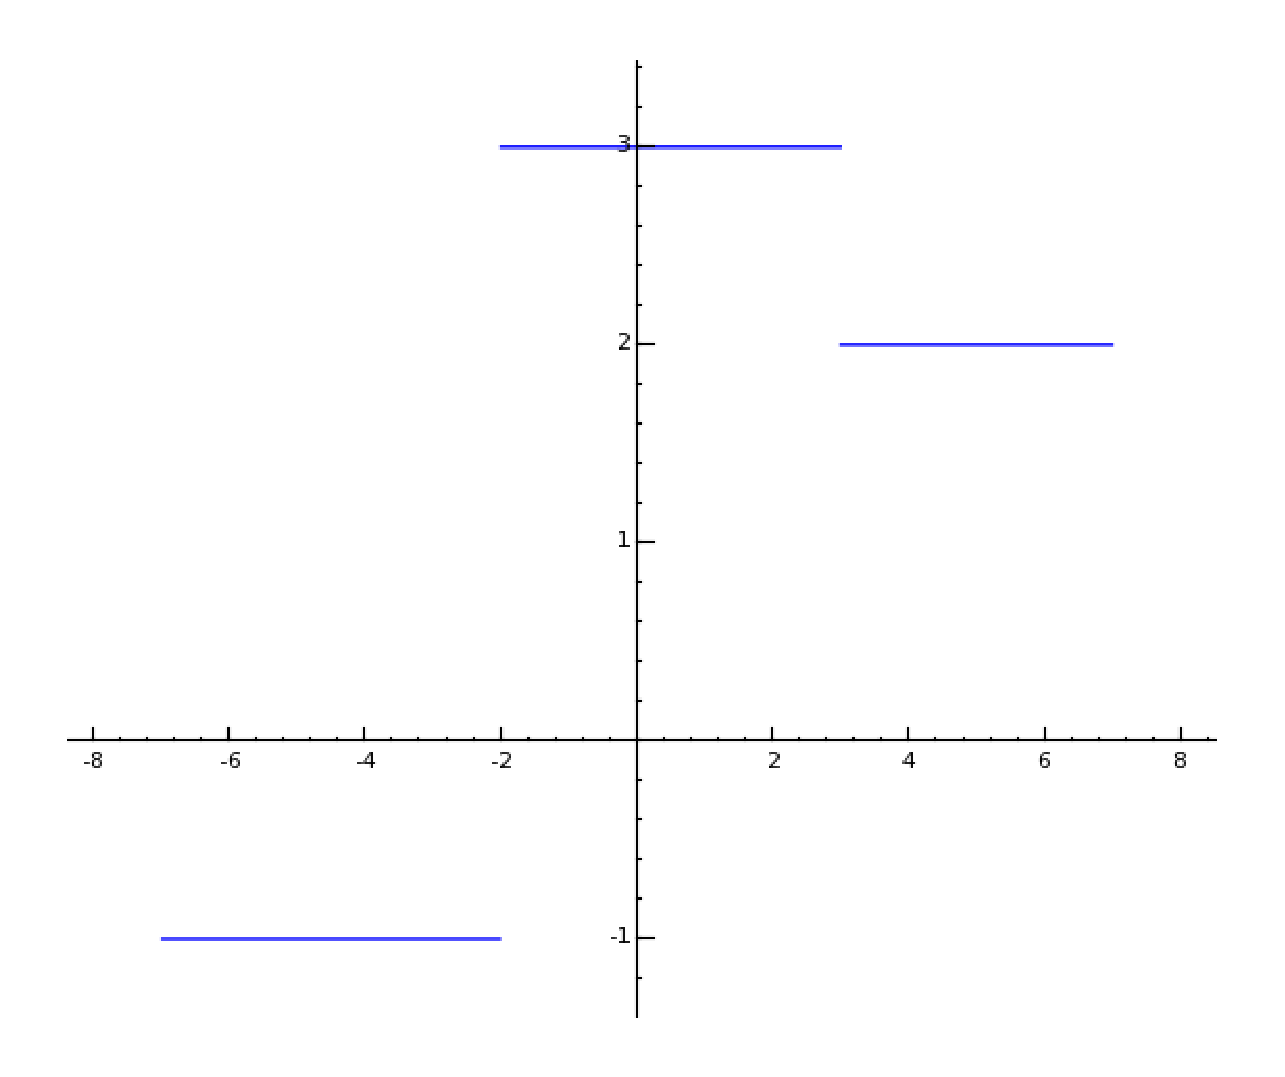
\includegraphics[height=4cm,width=8cm]{piecewise2.eps}
\end{center}
\caption{Another piecewise defined function.}
\label{fig:piecewise2}
\end{figure}
%sage: f1 = lambda x: -1
%sage: f2 = lambda x: 3
%sage: f3 = lambda x: 2
%sage: f = piecewise([[(-7,-2),f1],[(-2,3),f2],[(3,7),f3]])
%sage: P = f.plot()
%sage: show(P)

\end{enumerate}

Functions exist which are discontinuous for every value of the 
independent variable within a certain range. In the ordinary 
applications of the Calculus, however, we deal with functions 
which are discontinuous (if at all) only for certain isolated 
values of the independent variable; such functions are therefore 
in general continuous, and are the only ones considered in this book.

\section{Fundamental theorems on limits}
%20
\label{sec:20}

In problems involving limits the use of one or more of the 
following theorems is usually implied. It is assumed that the 
limit of each variable exists and is finite.

\begin{theorem}
{\rm 
%I. 
\label{thrm:I-20}
The limit of the algebraic sum of a finite number of 
variables is equal to the algebraic sum of the 
limits of the several variables. 

%% new
In particular,
\[
\lim_{x\to a} [f(x)+g(x)] = \lim_{x\to a} f(x)
+\lim_{x\to a} g(x).
\]
}
\end{theorem}

\begin{theorem}
{\rm
%II. 
\label{thrm:II-20}
The limit of the product of a finite number of variables is 
equal to the product of the limits of the several variables.

%% new
In particular,
\[
\lim_{x\to a} [f(x)\cdot g(x)] = \lim_{x\to a} f(x)
\cdot \lim_{x\to a} g(x).
\]
}
\end{theorem}

\begin{theorem}
{\rm
% III. 
\label{thrm:III-20}
The limit of the quotient of two variables is equal to the 
quotient of the limits of the separate variables, provided the 
limit of the denominator is not zero.

%% new
In particular,
\[
\lim_{x\to a} [f(x)/g(x)] = \frac{\lim_{x\to a} f(x)}{\lim_{x\to a} g(x)},
\]
provided $\lim_{x\to a} g(x)\not= 0$.
}
\end{theorem}

Before proving these theorems it is necessary to establish 
the following properties of infinitesimals.

\begin{enumerate}
\item
%(1) 
The sum of a finite number of infinitesimals is an 
infinitesimal. To prove this we must show that the 
numerical\footnote{In this book, the term ``numerical''
often is synonymous with ``absolute'' and  ``numerically''
often is synonymous with ``in absolute value''.}
value of this sum can be made less than any small positive 
quantity (as $\epsilon$) that may be assigned 
(\S \ref {sec:15}). That this is possible 
is evident, for, the limit of each infinitesimal being zero, 
each one can be made numerically less than $\frac{\epsilon}{n}$ 
($n$ being the number of infinitesimals), and therefore their sum 
can be made numerically less than $\epsilon$.

\item
%(2) 
The product of a constant $c\not= 0$ and an infinitesimal is an infinitesimal. 
For the numerical value of the product can always be made less 
than any small positive quantity (as $\epsilon$) by making the numerical 
value of the infinitesimal less than $\frac{\epsilon}{|c|}$.

\item
%(4) - reordered
If $v$ is a variable which approaches a limit $L$ different from zero, 
then the quotient of an infinitesimal by $v$ is also an 
infinitesimal. For if %limit $v = L$
$v\to L$, %% new 
and $k$ is any number numerically 
less than $L$, then, by definition of a limit, $v$ will ultimately become 
and remain numerically greater than $k$. Hence the quotient 
$\frac{\epsilon}{v}$, where $\epsilon$ is an infinitesimal, will ultimately 
become and remain numerically less than $\frac{\epsilon}{k}$, and is 
therefore by % (2)
%% new
the previous item
an infinitesimal.

\item
%(3) - reordered
The product of any finite number of infinitesimals is an 
infinitesimal. For the numerical value of the product may be 
made less than any small positive quantity that can be assigned. 
If the given product contains $n$ factors, then since each 
infinitesimal may be assumed less than the $n-th$ root of $\epsilon$, the 
product can be made less than $\epsilon$ itself.


\end{enumerate}

{\it Proof of Theorem \ref{thrm:I-20}.} 
Let $v_1$, $v_2$, $v_3$, $\dots$ be the variables, and 
$L_1$, $L_2$, $L_3$, $\dots$ their respective limits. We may then write

\[
v_1 - L_1 	= \epsilon_1,\ \ 
v_2 - L_2 	= \epsilon_2,\ \ 
v_3 - L_3 	= \epsilon_3,
\]
where $\epsilon_1$, $\epsilon_2$, $\epsilon_3$, $\dots$ are 
infinitesimals (i.e. variables having zero for a limit). Adding

\[
%(A) 
(v_1 + v _2 + v_3 + \dots) - (L_1 + L_2 + L_3 + . . .) 
= (\epsilon_1 + \epsilon_2 + \epsilon_3 + \dots).
\]
Since the right-hand member is an infinitesimal by item
(1) above (\S \ref{sec:20}), 
we have, from the converse theorem (\S \ref{sec:15}),

\[
  	\lim (v_1 + v_2 + v_3 + \dots) 
= L_1 + L_2 + L_3 + \dots,
\]
or, 	

\[
\lim (v_1 + v_2 + v_3 + \dots) 
= \lim v_1 + \lim v_2 + \lim v_3 + \dots,
\]
which was to be proved. \qed


{\it Proof of Theorem \ref{thrm:II-20}.} 
Let $v_1$ and $v_2$ be the variables, $L_1$ and $L_2$ their 
respective limits, and $\epsilon_1$ and $\epsilon_2$ infinitesimals; 
then
\[
  	v_1 	= L_1 + \epsilon_1
\]
and $v_2 = L_2 + \epsilon_2$.
Multiplying, 

\[
\begin{array}
{ll}
v_1v_2 	&= (L_1 + \epsilon_1)(L_2 + \epsilon_2)\\
&	= L_1L_2 + L_1\epsilon_2 + L_2\epsilon_1 + \epsilon_1\epsilon_2
\end{array}
\]
or, 	  	 

\[
v_1v_2 - L_1L_2 = L_1\epsilon_2 + L_2\epsilon_1 + \epsilon_1\epsilon_2.
\]
Since the right-hand member is an infinitesimal 
by items (1) and (2) above, (\S \ref{sec:20}), we have, as before,

\[
\lim (v_1v_2) = L_1L_2 = \lim v_1 \cdot \lim v_2,
\]
which was to be proved. \qed

{\it Proof of Theorem \ref{thrm:III-20}.}  
Using the same notation as before,

\[
  \frac{v_1}{v_2} = \frac{L_1 + \epsilon_1}{L_2 + \epsilon_2} 
= \frac{L_1}{L_2} + \left ( \frac{L_1 + \epsilon_1}{L_2 + \epsilon_2} 
- \frac{L_1}{L_2} \right ),
\]
or,

\[
\frac{v_1}{v_2} - \frac{L_1}{L_2} 
= \frac{L_2 \epsilon_1 - L_1 \epsilon_2}{L_2 (L_2 + \epsilon_2)}.
\]
Here again the right-hand member is an infinitesimal 
by item (3) above, (\S \ref{sec:20}), if $L_2 \ne 0$; hence

\[
\lim \left ( \frac{v_1}{v_2} \right ) = \frac{L_1}{L_2} 
= \frac{\lim\,v_1}{\lim\,v_2},
\]
which was to be proved. \qed

It is evident that if any of the variables be 
replaced by constants, our reasoning still holds, and 
the above theorems are true.

\section{Special limiting values}
%21

The following examples are of special importance in the 
study of the Calculus. In the following examples $a > 0$ and 
$c \ne 0$.

\vskip .2in
\begin{center}
\begin{tabular}{lcc}
Eqn number & Written in the form of limits & 	Abbreviated form often used \\ \hline
(1) &	$\lim_{x \to 0} \frac{c}{x} 	= \infty$ & 	 $\frac{c}{0} 	= \infty$\\
 & & \\
(2) &	$\lim_{x \to \infty} cx 	= \infty$         & 	  $c \cdot \infty 	= \infty$ \\
 & & \\
(3) &	$\lim_{x \to \infty} \frac{x}{c} 	= \infty$ & $\frac{\infty}{c} 	= \infty$ \\
 & & \\
(4) &	$\lim_{x \to \infty} \frac{c}{x} 	= 0$      & $\frac{c}{\infty} 	= 0$ \\
 & & \\
(5) &	$\lim_{x \to -\infty} a^x, 	= +\infty$ , 	when $a < 1$ & $ a^{-\infty} 	= +\infty$ \\
 & & \\
(6) &	$\lim_{x \to +\infty} a^x 	= 0$, 	when $a < 1$         & 	$a^{+\infty} 	= 0$ \\
 & & \\
(7) &	$\lim_{x \to -\infty} a^x 	= 0$, 	when $a > 1$         & 	$a^{-\infty} 	= 0$ \\
 & & \\
(8) &	$\lim_{x \to +\infty} a^x 	= +\infty$, 	when $a > 1$ & 	$a^{+\infty} 	= +\infty$\\
 & & \\
(9) &	$\lim_{x \to 0} \log_a\ x 	= +\infty$, 	when $a < 1$ & 	$\log_a\ 0 	= +\infty$ \\
 & & \\
(10)& 	$\lim_{x \to +\infty} \log_a\ x 	= -\infty$, 	when $a < 1$ & $\log_a(+\infty) 	= -\infty$ \\
 & & \\
(11)& 	$\lim_{x \to 0} \log_a\ x 	= -\infty$, 	when $a > 1$ & $\log_a\ 0 	= -\infty$ \\
 & & \\
(12)& 	$\lim_{x \to +\infty} \log_a\ x 	= +\infty$, 	when $a > 1$ & $\log_a(+\infty) 	= +\infty$ \\
\end{tabular}
\end{center}

The expressions in the %second 
last % new
column are not to be considered as expressing numerical 
equalities ($\infty$ not being a number); they are merely symbolical equations 
implying the relations indicated in the first column, and should be so understood.

% 22
\section{Show that $\lim_{x \to 0} \frac{\sin\, x}{x} = 1$}
\label{sec:22}

To motivate the limit computation of this section, using \sage 
we compute a number of values of the function
$\frac{\sin\, x}{x}$, as $x$ gets closer and closer to $0$:

\vskip .1in

\begin{center}
\begin{tabular}{l|lllll}
$x$ & 0.5000 & 0.2500 & 0.1250 & 0.06250 & 0.03125\\ \hline
$\frac{\sin(x)}{x}$ & 0.9589 & 0.9896 & 0.9974 & 0.9994 & 0.9998\\
\end{tabular}
\end{center}
%sage: f = lambda x: sin(x)/x
%sage: R = RealField(15)
%sage: [R(x) for x in L]
%[0.5000, 0.2500, 0.1250, 0.06250, 0.03125]
%sage: [R(f(x)) for x in L]
%[0.9589, 0.9896, 0.9974, 0.9994, 0.9998]

\vskip .1in

\noindent
Indeed, if we refer to the table %on p. 4 [§ 4],
in \S \ref{sec:4},
it will be seen that for all angles less than $10^o$ the angle in radians 
and the sine of that angle are equal to three decimal places. 
To compute the table of values above using \sage, simply use the 
following commands.


\vskip .1in

\begin{Verbatim}[fontsize=\small,fontfamily=courier,fontshape=tt,frame=single,label=\sage]

sage: f = lambda x: sin(x)/x
sage: R = RealField(15)
sage: L = [1/2^i for i in range(1,6)]; L
[1/2, 1/4, 1/8, 1/16, 1/32]
sage: [R(x) for x in L]
[0.5000, 0.2500, 0.1250, 0.06250, 0.03125]
sage: [R(f(x)) for x in L]
[0.9589, 0.9896, 0.9974, 0.9994, 0.9998]

\end{Verbatim}
\vskip .1in

\noindent
From this we may well suspect that
$ \lim_{x \to 0} \frac{\sin\, x}{x} = 1$.

Let $O$ be the center of a circle whose radius is unity.

Let $\operatorname{arc}\ AM = \operatorname{arc}\ AM' = x$, and let 
$MT$ and $M'T$ 
be tangents drawn to the circle at $M$ and $M'$. From Geometry 
(see Figure \ref{fig:limit-proof}), % new

\begin{figure}[h!]
\begin{minipage}{\textwidth}
\begin{center}
%\vspace{1.0 cm}
%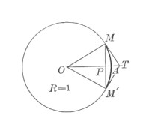
\includegraphics[height=4cm,width=4cm]{limit_proof.eps}
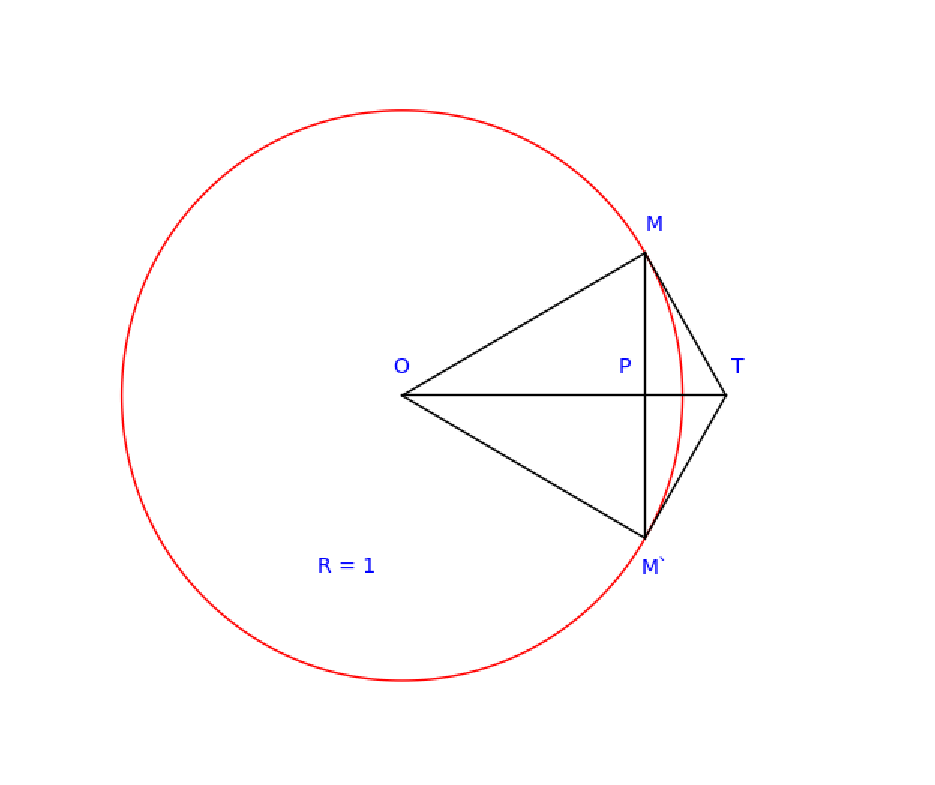
\includegraphics[height=5cm,width=6cm]{circle-tangent.eps}
\end{center}
\end{minipage}
%\caption{Scan of Granville's unit circle.}
\caption{Comparing $x$ and $\sin(x)$ on the unit circle.}
\label{fig:limit-proof}
\end{figure}
%sage: c = circle((0,0), 1, rgbcolor=(1,0,0))
%sage: P1 = line([(sqrt(3)/2,1/2),(2/sqrt(3),0)], rgbcolor=(0,0,0))
%sage: P2 = line([(sqrt(3)/2,-1/2),(2/sqrt(3),0)], rgbcolor=(0,0,0))
%sage: P3 = line([(sqrt(3)/2,-1/2),(sqrt(3)/2,1/2)], rgbcolor=(0,0,0))
%sage: P4 = line([(0,0),(sqrt(3)/2,1/2)], rgbcolor=(0,0,0))
%sage: P5 = line([(0,0),(sqrt(3)/2,-1/2)], rgbcolor=(0,0,0))
%sage: P6 = line([(0,0),(2/sqrt(3),0)], rgbcolor=(0,0,0))
%sage: t1 = text('T', (1.2, 0.1))
%sage: t2 = text('M', (0.9, 0.6))
%sage: t3 = text('M`', (0.9, -0.6))
%sage: t4 = text('P', (0.8, 0.1))
%sage: t5 = text('O', (0.0, 0.1))
%sage: t6 = text('R = 1', (-0.2, -0.6))
%sage: show(c+P1+P2+P3+P4+P5+P6+t1+t2+t3+t4+t5+t6,axes=False)

%\newpage

\noindent
we have % new
\[
MPM' < MAM' < MTM';
\]
or $2 \sin\, x < 2x < 2 \tan\ x$.
Dividing through by $2 \sin\, x$, we get

\[
    1 < \frac{x}{\sin\, x} < \frac{1}{\cos\ x}.
\]
If now $x$ approaches the limit zero,

\[
    \lim_{x \to 0} \frac{x}{\sin\, x}
\]
must lie between the constant $1$ and $\lim_{x \to 0} \frac{1}{\cos\ x}$, which is also $1$.
Therefore $\lim_{x \to 0} \frac{x}{\sin\, x} = 1$, or, 
$\lim_{x \to 0} \frac{\sin\, x}{x} = 1$ Theorem \ref{thrm:III-20}.
\qed

It is interesting to note the behavior of this function from its graph, the locus of equation
\[
    y = \frac{\sin\, x}{x}
\]
\begin{figure}[h!]
\begin{minipage}{\textwidth}
\begin{center}
%\vspace{1.0 cm}
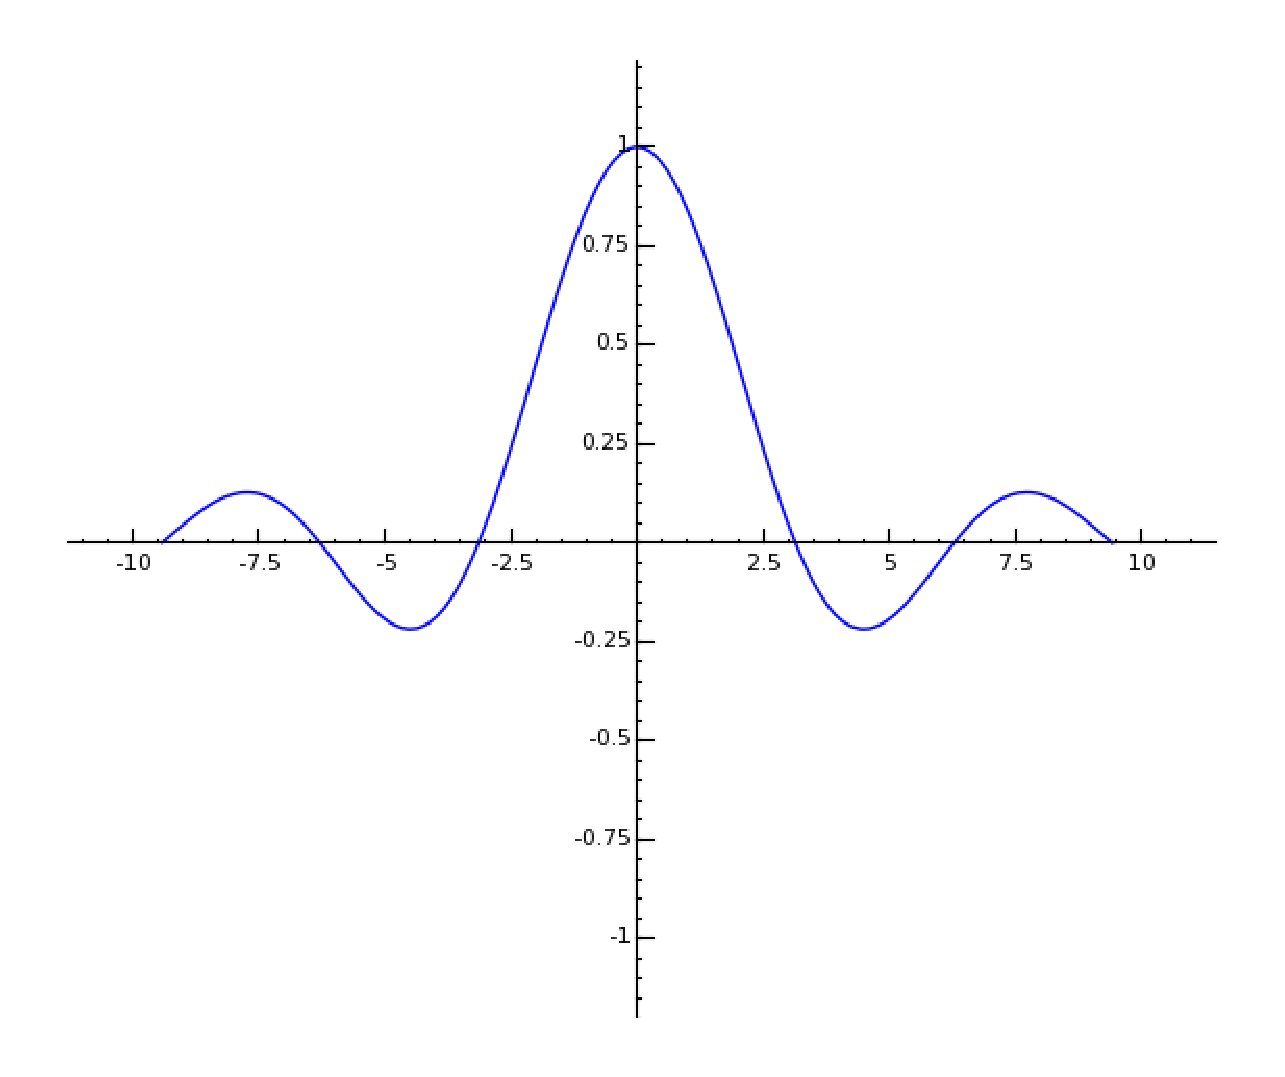
\includegraphics[height=4cm,width=8cm]{limit_proof2.eps}
\end{center}
\end{minipage}
\caption{The function $\frac{\sin(x)}{x}$.}
\label{fig:limit-proof2}
\end{figure}
%sage: P = plot(sin(x)/x,-3*pi,3*pi)
%sage: show(P)

Although the function is not defined for $x = 0$, yet it is not discontinuous 
when $x = 0$ if we define $ \frac{\sin\, 0}{0} = 1$ (see Case II in \S \ref{sec:18}).

Finally, we show how to use the \sage command {\tt limit} to compute the 
limit above\footnote{We use the command-line version of \sage, as opposed
to the GUI notebook version. The commands are the same for the GUI version.}.


\vskip .1in

\begin{Verbatim}[fontsize=\small,fontfamily=courier,fontshape=tt,frame=single,label=\sage]

sage: limit(sin(x)/x,x=0)
1

\end{Verbatim}


%23. 
\section{The number $e$}
\label{sec:23}

One of the most important limits in the Calculus is

\[
    \lim_{x \to 0} (1 + x)^{\frac{1}{x}} = 2.71828\cdots = e
\]
To prove rigorously that such a limit $e$ exists, is beyond the scope of 
this book. For the present we shall content ourselves by plotting the locus of the equation

\[
    y = (1 + x)^{\frac{1}{x}}
\]
and show graphically that, as $x \dot= 0$, the function $(1 + x)^\frac{1}{x}(= y)$
takes on values in the near neighborhood of $2.718\dots$, and therefore 
$e = 2.718\dots$, approximately.

\begin{figure}[h!]
\begin{minipage}{\textwidth}
\begin{center}
%\vspace{1.0 cm}
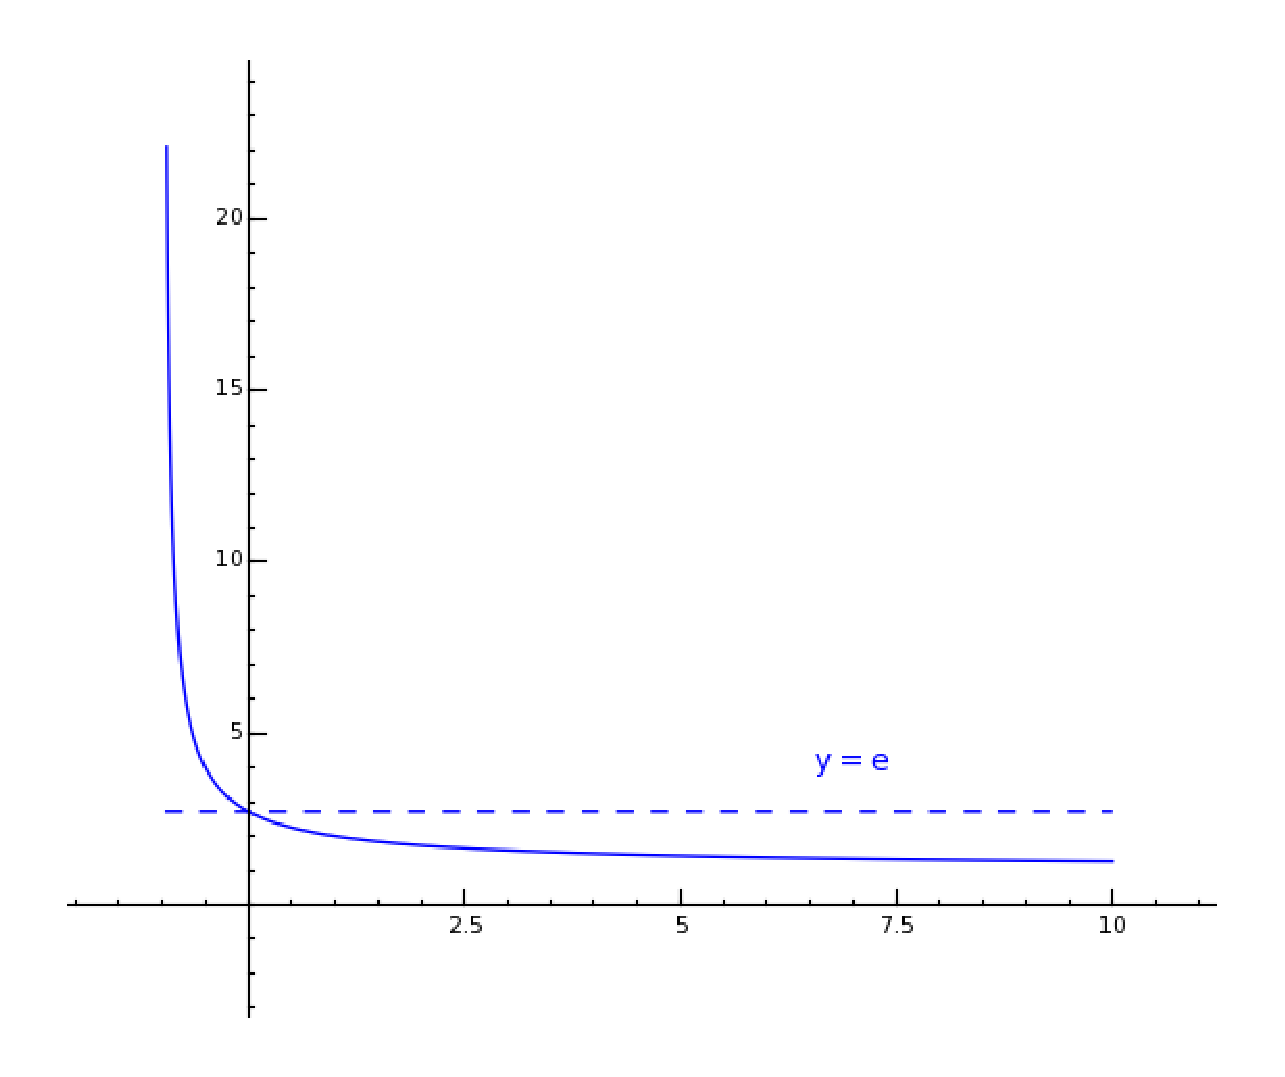
\includegraphics[height=4cm,width=8cm]{limite.eps}
\end{center}
\end{minipage}
\caption{The function $(1+x)^{1/x}$.}
\label{fig:limite}
\end{figure}
%sage: P1 = plot((1+x)^(1/x),-0.99,10)
%sage: P2 = plot(e^1,-0.99,10,linestyle="--")
%sage: P3 = text("y = e",(7,4))
%sage: show(P1+P2+P3)

\vskip .1in

{\scriptsize{
\begin{tabular}{c|cccccccccc}
$x$          %   & -1/2 
& -.1      %& -.01    
& -.001 & .001    & .01    &  .1    %& .50   
& 1 	&5 &10 	\\ \hline	
$y=(1+x)^{1/x}$  % &  4    
& 2.8680   %& 2.7320 
& 2.7195 & 2.7169 &	2.7048 & 2.5937 %& 2.250 
& 2.0000&1.4310&1.0096 \\
\end{tabular}
}}

\vskip .1in

As $x \to 0-$ from the left, $y$ decreases and approaches $e$ as a limit. 
As $x \to 0+$ from the right, $y$ increases and also approaches $e$ as a limit.

As $x \to \infty$, $y$ approaches the limit $1$; and as $x \to -1+$ from the right, $y$ 
increases without limit.

%In Chap. \ref{ch:XVIII}, Exercise 15, we will show how to calculate the value of 
%$e$ to any number of decimal places.

Natural logarithms are those which have the number $e$ for base. These logarithms 
play a very important rôle in mathematics. When the base is not indicated explicitly, 
the base $e$ is always understood in what follows in this book. Thus $\log_e\ v$ is written simply 
$\log\ v$ or $\ln\ v$.

Natural logarithms possess the following characteristic property: If $x \to 0$ in any way whatever,

\[
  \lim \frac{\log(1 + x)}{x} = \lim \log(1 + x)^{\frac{1}{x}} = \log\ e 
= \ln e %% new
= 1. 
\]

%24.
\section{Expressions assuming the form $\frac{\infty}{\infty}$} 
\label{sec:24}

As $\infty$ is not a number, the expression $\infty\ \div\ \infty$ is indeterminate. 
To evaluate a fraction assuming this form, the numerator and denominator 
being algebraic functions, we shall find useful the following

\noindent
{\bf RULE.} 
Divide both numerator and denominator by the highest power of the variable occurring in either. 
Then substitute the value of the variable.

\begin{example}
{\rm
%ILLUSTRATIVE EXAMPLE 1. 
Evaluate %\lim_{x \to \infty} \frac{2x^3 - 3x^2 + 4}{5x - x^2 - 7x^3}%.

Solution. Substituting directly, we get 

\[
\lim_{x \to \infty} \frac{2x^3 - 3x^2 + 4}{5x - x^2 - 7x^3} = \frac{\infty}{\infty}
\]
which is indeterminate. Hence, following the above rule, we divide both 
numerator and denominator by $x^3$, Then

\[
 \lim_{x \to \infty} \frac{2x^3 - 3x^2 + 4}{5x - x^2 - 7x^3} 
= \lim_{x \to \infty} \frac{2 - \frac{3}{x} + \frac{4}{x^3}}{\frac{5}{x^2} - \frac{1}{x} - 7} 
= -\frac{2}{7}.
\]
}
\end{example}

%\vskip .3in
%\begin{center}
%{\bf Exercises}
%\end{center}
%\vskip .2in

\section{Exercises}

Prove the following:
\begin{enumerate}
\item
%1. 
$\lim{x \to \infty} \left ( \frac{x + 1}{x} \right ) = 1$.

%Proof. 
Solution:

\[
\begin{array}{ll}
\lim_{x \to \infty} &	= \lim_{x \to \infty} \left ( 1 + \frac{1}{x} \right )\\
&  	= \lim_{x \to \infty} (1) + \lim{x \to \infty} \left ( \frac{1}{x} \right )   \\
 & 	= 1 + 0 = 1,
\end{array}
\]
by Theorem \ref{thrm:I-20}
%Th. I, p. 18 [§ 20]

%2.
\item
$ \lim_{x \to \infty} \left ( \frac{x^2 + 2x}{5 - 3x^2} \right ) = -\frac{1}{3}$.

%Proof. 
Solution:

\[
\lim_{x \to \infty} \left ( \frac{x^2 + 2x}{5 - 3x^2} \right ) 	
= \lim_{x \to \infty} \left ( \frac{1 + \frac{2}{x}}{\frac{5}{x^2} - 3} \right )
\]
[ Dividing both numerator and denominator by $x^2$.]
\[
= \frac{\lim_{x \to \infty} \left ( 1 + \frac{2}{x} \right )}{\lim_{x \to \infty} 
\left ( \frac{5}{x^2} - 3 \right )}  
\]
by Theorem \ref{thrm:III-20}
% Th. III, p. 18 [§ 20]
\[
 	= \frac{\lim_{x \to \infty} (1) + \lim_{x \to \infty} \left ( \frac{2}{x} \right ) }{ \lim_{x \to \infty} \left ( \frac{5}{x^2} \right ) - \lim_{x \to \infty} (3)}   
  	= \frac{1 + 0}{0 - 3} = -\frac{1}{3},
\]
by Theorem \ref{thrm:I-20}.
%Th. I, p. 18 [§ 20]

%3.
\item
$ \lim_{x \to 1} \frac{x^2 - 2x + 5}{x^2 + 7} = \frac{1}{2}$.

%4.
\item
$ \lim_{x \to 0} \frac{3x^3 + 6x^2}{2x^4 - 15x^2} = -\frac{2}{5}$.

%5.
\item
$ \lim_{x \to -2} \frac{x^2 + 1}{x + 3} = 5$.

%6.
\item
$ \lim_{h \to 0} (3ax^2 - 2hx + 5h^2) = 3ax^2$.

%7.
\item
$ \lim_{x \to \infty} (ax^2 + bx + c) = \infty$.

%8.
\item
$ \lim_{k \to 0} \frac{(x - k)^2 - 2kx^3}{x(x + k)} = 1$.

%9.
\item
$ \lim_{x \to \infty} \frac{x^2 + 1}{3x^2 + 2x - 1} = \frac{1}{3}$.

%10.
\item
$ \lim_{x \to \infty} \frac{3 + 2x}{x^2 - 5x} = 0$.

%11.
\item
$ \lim_{\alpha \to \frac{\pi}{2}} \frac{\cos(\alpha - a)}{\cos(2\alpha - a)} = -\tan \alpha$.

%12.
\item
$ \lim_{x \to \infty} \frac{ax^2 + bx + c}{dx^2 + ex + f} = \frac{a}{d}$.

%13.
\item
$ \lim_{z \to 0} \frac{a}{2} (e^{\frac{z}{a}} + e^{-\frac{z}{a}}) = a$.

%14.
\item
$ \lim_{x \to 0} \frac{2x^3 + 3x^2}{x^3} = \infty$.

%15.
\item
$  \lim_{x \to \infty} \frac{5x^2 - 2x}{x} = \infty$.

%16.
\item
$  \lim_{y \to \infty} \frac{y}{y + 1} = 1$.

%17.
\item
$  \lim_{n \to \infty} \frac{n(n + 1)}{(n + 2)(n + 3)} = 1$.

%18.
\item
$  \lim_{s \to 1} \frac{s^3 - 1}{s - 1} = 3$.

%19.
\item
$  \lim_{h \to 0} \frac{(x + h)^n - x^n}{h} = nx^{n-1}$.

%20.
\item
$  \lim_{h = 0} \left [ \cos(\theta + h) \frac{\sin h}{h} \right ] = \cos \theta$.

%21.
\item
$  \lim_{x \to \infty} \frac{4x^2 - x}{4 - 3x^2} = -\frac{4}{3}$.

%22.
\item
$  \lim_{\theta \to 0} \frac{1 - \cos \theta}{\theta^2} = \frac{1}{2}$.

%23.
\item
$  \lim_{x \to a} \frac{1}{x - a} = -\infty$, if $x$ is increasing as it approaches the value $a$.

%24.
\item
$  \lim_{x \to a} \frac{1}{x - a} = +\infty$, if $x$ is decreasing as it approaches the value $a$.
\end{enumerate}

\vskip .1in

Here is an example of the limit in Exercise 22 using \sage:

\vskip .2in

\begin{Verbatim}[fontsize=\scriptsize,fontfamily=courier,fontshape=tt,frame=single,label=\sage]

sage: theta = var("theta")
sage: limit((1 - cos(theta))/(theta^2),theta=0)
1/2

\end{Verbatim}

\vskip .1in
\noindent
In other words, for small values of $\theta$,
$
\cos(\theta) \cong 1+\frac{1}{2}\theta^2.
$
